% !TeX root = ../main-paper.tex
\section{Experiment 2: Impact of OCR noise on named entity recognition}
\label{sec:ner-xp2}
Noise introduced by OCR is known to have a negative impact on NER, because it alters the structure and lexicon of the input texts, moving them away from the language model known to the NER process.
In real-life situations, the models are often trained on texts without such noise, even though the texts to be annotated are extracted with OCR.
In this second experiment, we aim at assessing the most appropriate strategy to build a NER model tolerant to OCR noise.


\subsection{Training and evaluation protocol}
Only CmBERT and CmBERT+ptrn are considered since experiment 1 shows that SpaCy NER is systematically outperformed by these two models.

We leverage the labeled sets of entries NER-\emph{reference}, NER-\emph{pero} and NER-\emph{tesseract} created as explained in \cref{sec:dataset}.
Kraken is left aside as it produces poor results that would require removing 500 entries from all datasets to keep the same set of valid entries.

Each dataset is split into training development, and test sets following the same protocol as described in \cref{sec:ner-xp1-protocol}, except this time we do not need to create smaller training sets.
As the NER sets contain 8341 entries, the produced train sets (resp. development and test) contain 6004 entries - 72\% of the total (resp. 668 - 8\% and 1669 - 20\%).    

CmBERT and CmBERT+ptrn are fine-tuned on the training sets built from NER-\emph{reference} and NER-\emph{pero}.
The training parameters are mostly the same as in \cref{sec:ner-xp1-protocol}, only this time the patience threshold is set to 5 evaluations.
Finally the metrics are measured against the three tests sets.




%\subsubsection{Huggingface CamemBERT}
%\joseph{Copie de \cref{sub:ner-xp1-sysytems-huggingcam}. Je suggère de rédiger la section de l'XP 1 en premier et apporter précision nécessaires ici.}

%Experiments 1 and 2 rely on the implementation of transformers provided by the software library Huggingface (transformers v.4.15.0, datasets v.1.17.0).
%Our baseline CmBERT model is CamemBERT model published on the Hugging Face repository \footnote{\url{https://huggingface.co/Jean-Baptiste/camembert-ner}} and already trained for NER on wikiner-fr.
%Its NER head is a linear model with a Softmax function.
%CmBERT and CmBERT+ptrn are always fine-tuned using the same parameters, with at most 5000 training steps and an early stopping condition set to 3 evaluations in experiment 1 (5 in experiment 2) without improvement of the f1 score. Evaluations are performed every 100 steps.

%\subsection{Protocol}

%We fine-tune CmBERT and CmBERT+ptrn on reference-gold and pero-gold to create two versions of each model: the former trained on manually corrected entries and the latter on OCR entries.
%SpaCy NER is left aside as results from experiment 1 show that it is outperformed by BERT models.
%Performance metrics are computed for each of the four resulting NER models against the test sets created from reference-gold, pero-gold and tesseract-gold.


\subsection{Results and discussion}
The measured F1-score are given in \cref{fig:exp_2_eval_ner}.
Results clearly show that models perform best when both the pre-training and the NER fine-tuning share the same characteristics (here, OCR noise) as the texts to be processed.

In our tests, pre-training the model brings a slight gain in performance ($\approx 0.5\%$).
We did not pre-train or fine-tune with texts extracted with Tesseract.
However, despite a loss of performance, the model pre-trained and fine-tuned on NER-pero still gives the best results.
This is probably due to the fact that the texts produced by Pero-OCR feature characteristics intermediary between human transcriptions and Tesseract.
This OCR tool removes the characters recognised with low confidence, which is probably a great help to the NER.

\begin{figure}
    \centering
    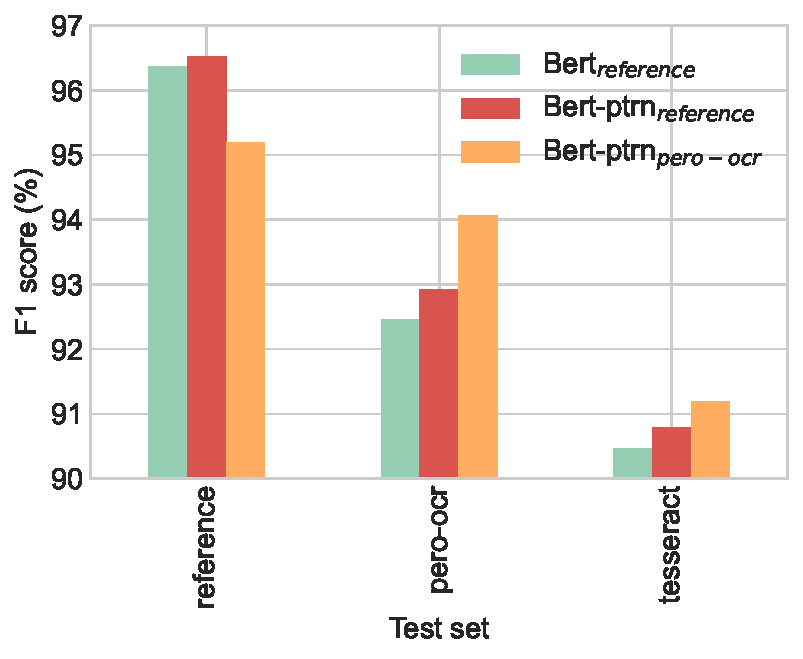
\includegraphics[width=0.75\textwidth]{images/experiment_2_f1_with_noise_graph.pdf}
    \caption{\label{fig:exp_2_eval_ner}NER F1-scores in presence of OCR noise in the training and testing examples, grouped by test set. The dataset used to train the NER task is noted in indice after the model name (e.g. CmBERT$_{pero}$ means CmBERT fine-tuned on NER-\emph{pero}).}
\end{figure}

